To demonstrate how CrowdNote works, an instance was created to enrich the videos by incorporating extra content such as images, text boxes, Wikipedia content, and Youtube videos. In order to enrich the videos, it was decided that the crowd should to identify which points of interest in the video, suggest content to associate with them, select the best suggestions, and finally determine the position in the videos where they should be displayed.

Thus, 4 simple microtasks of annotation were defined, which when cascaded would generate the complex annotations necessary for enrichment. These annotations consist of the list of content that should be displayed in each interval of the video, as well as the position in which they should be displayed. In addition, for each microtask, was defined the appropriate aggregation method to generate input for the next one, as so to generate the final outcome.


\begin{itemize}
\item \textbf{Task 1 - Identify the points of interest} on the video that should be associated with extra content. The aggregation method proceed a temporal grouping over the contributions. For each group, a content analysis is performed to merge equivalent contributions. Finally, the predominant entry is selected in each group, and marked as the point of interest at that time in relation to the timeline.

\item \textbf{Task 2: Provide extra content suggestions} for each point of interest. In the aggregation, the content provided by contributors is grouped by point of interest. Therefore, a content analysis is done to group equivalent contributions.

\item \textbf{Task 3: Ranking the suggested content} provided by each point of interest. The contributors elect the suggested content that better complement each point of interest. In the aggregation, the most popular suggestion for each point of interest is selected based on contributions to task 3.
	
\item \textbf{Task 4: Determine the positions} to display the extra content associated with each point of interest. The contributors suggest the position for each content and, in the aggregation, the contributions are grouped by point of interest and, for each point, the average coordinate is determined.

\end{itemize}

\subsection{Cascading Microtasks}
The adopted approach consists in divide the complex annotation into simple annotations that can be collected by 
a set of simple annotation tools. Each of these simple annotations are collected by a microtask.

How is illustrated in Figure~\ref{cascading}, the input for each task is generated by the Aggregator after the previous task, except for the task 1. For this task is provided a bootstrap Input that is a list of video segments provided by the owner, that is who initiate the process. Each entry of the bootstrap input can represent a semantic block of the video. 

\begin{figure}[h!]
 \centerline{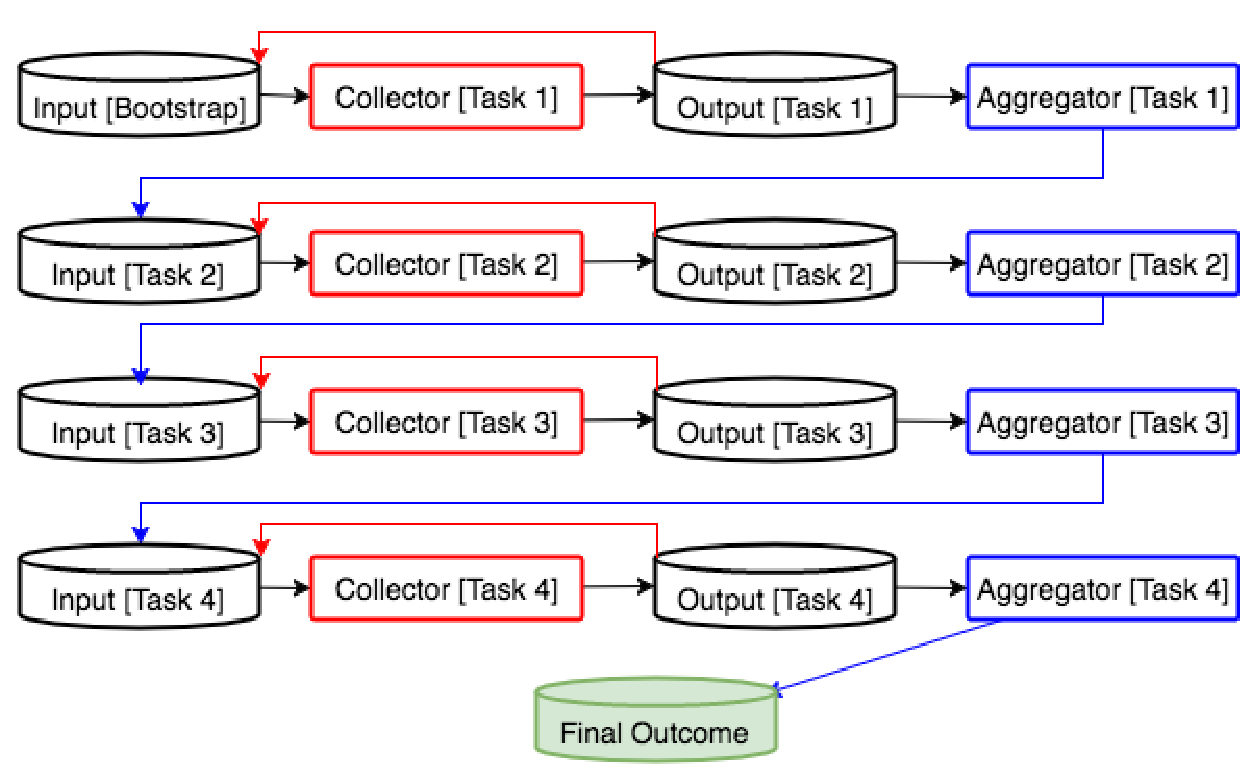
\includegraphics[scale=0.35] {figure/Cascading}}
	\caption{Cascading Microtasks}
	\label{cascading}
\end{figure}

Other applications that use CrowdNote may use different strategies to segment videos such as fixed time-length, SRT files, or even add a microtask to segment videos.
		


\subsection{Task 1}
\textbf{Identify Points of Interest:} The first annotation microtask is supported by the tool represented in Figure~\ref{task_1}, collecting identification for points of interest. In this task the contributor receive a segment of video that should be watched, and if was found any point of interest, it should be marked and briefly described. These points of interest can be gestures, words, expressions, facts, concept, characters, events or anything that can be related to extra content.

\begin{figure}[h!]
	\centerline{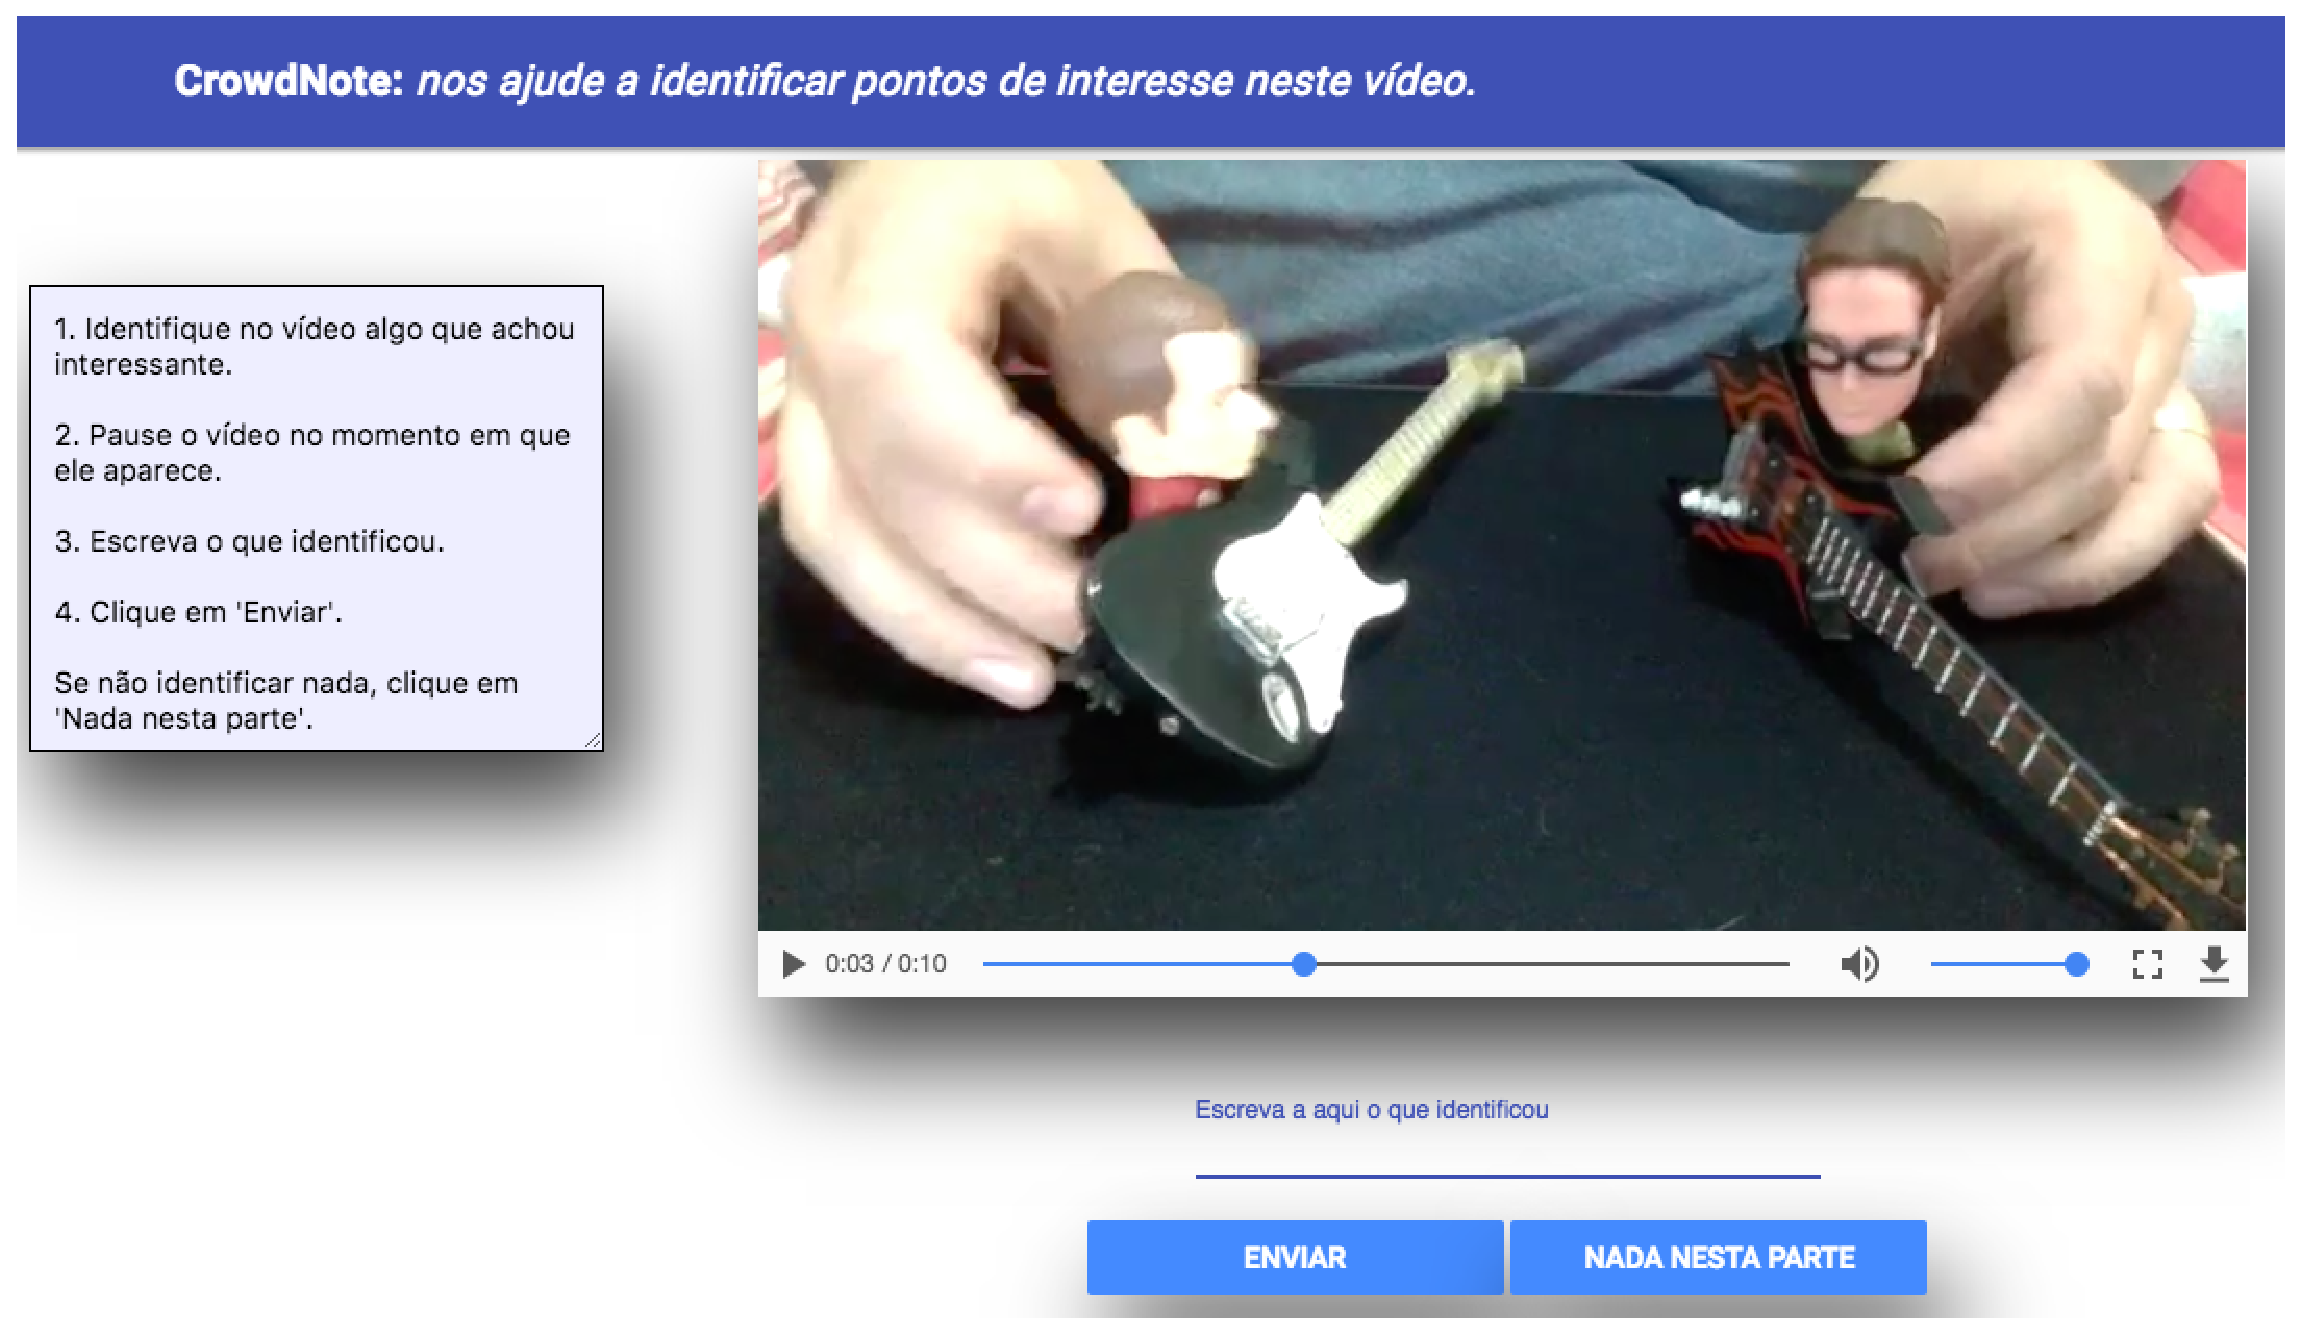
\includegraphics[scale=0.22] {figure/task_1}}
	\caption{Task 1}
	\label{task_1}
\end{figure}

\subsection{Task 2}

\textbf{Provide extra content suggestions:} The second task taken as input the aggregated result from the task 1 and is supported by the annotation tool represented in Figure~\ref{task_2}. In this task the contributor receive a video segment and a text describing  the point of interest to be observed, and must suggest an extra content to be associated with the point of interest. The extra content can be an image, a text, a hyperlink for a Youtube video, or a hyperlink to a Wikipedia page. 

\begin{figure}[h!]
	\centerline{\includegraphics[scale=0.18] {figure/task_2}}
	\caption{Task 2}
	\label{task_2}
\end{figure}

After the aggregation the outcome from this task is a set of points of interest, and a list of suggests of extra content to be related to each one of them.


\subsection{Task 3}

\textbf{Ranking Suggestions:} The third microtask aimed ranking the suggested contents that resulted from the task 2. The job consists in presenting to the worker a point of interest and the suggested contents related to it. The worker must select which content seems most appropriate to determine the point of interest. This task is supported by the annotation tool represented in Figure~\ref{task_3}.

		
\begin{figure}[h!]
	\centerline{\includegraphics[scale=0.22] {figure/task_3}}
	\caption{Task 3}
	\label{task_3}
\end{figure}

The aggregation process for this task checks which suggestions are most popular among the contributors and selects them to enrich the video.

\subsection{Task 4}

\textbf{Determine the positions:} The last task is to determine the position in the video where the extra content for each point of interest should be displayed. The correct position of each extra content is important to avoid occlusion and display content pleasingly to the user.

Following the studies about wisdom  of the crowd, the strategy to determine the correct position is to calculate the average coordinate of the contribution for each content \citep{GALTON1907}. The annotation tool represented in Figure~\ref{task_4} made this microtask faster and easier between the 4 tasks.

\begin{figure}[h!]
	\centerline{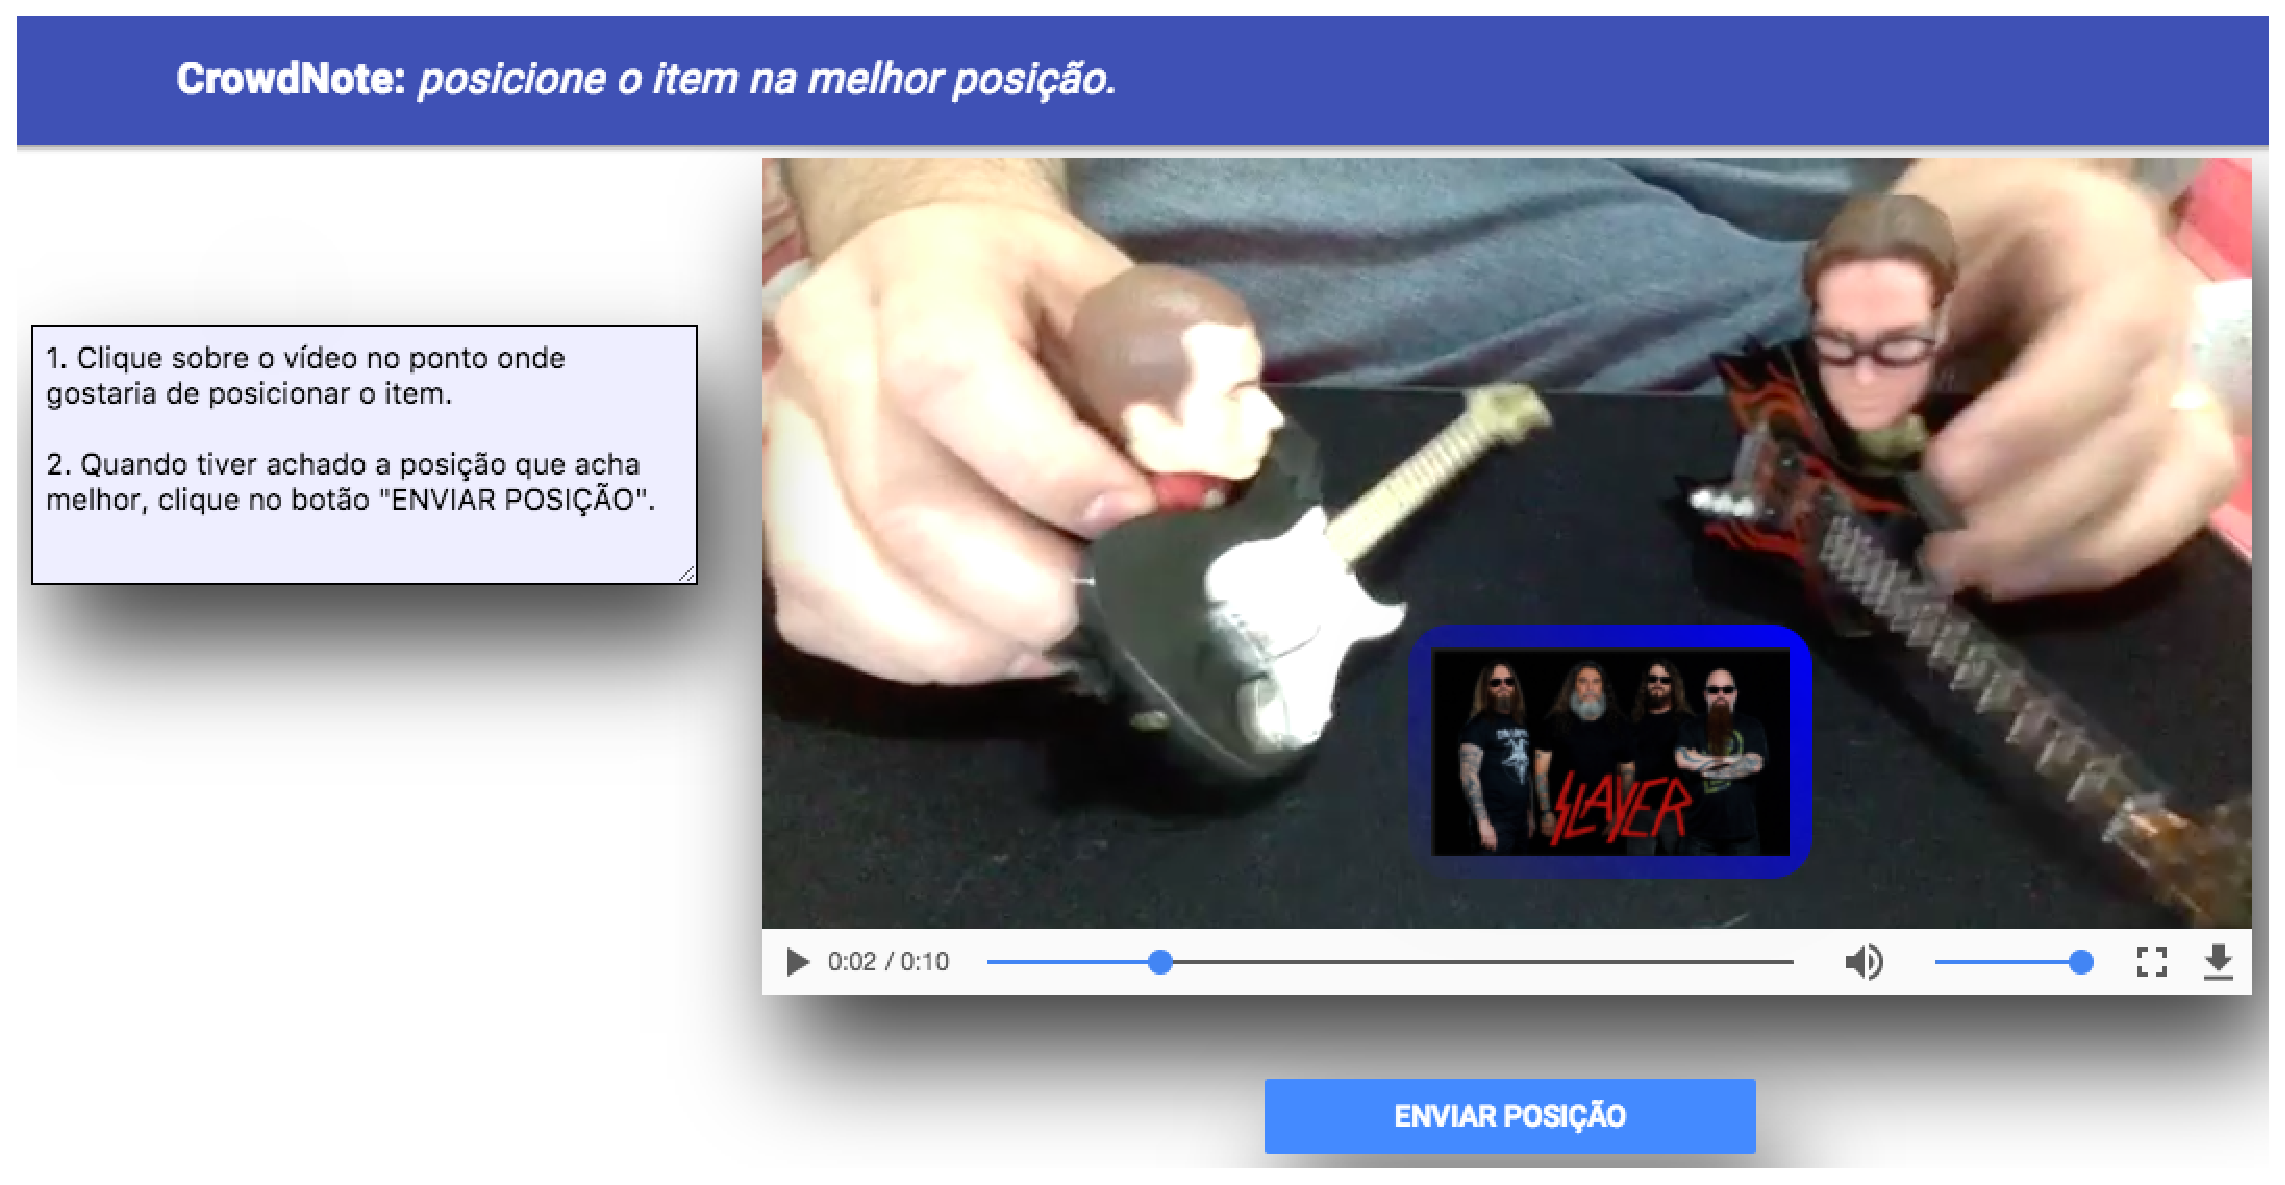
\includegraphics[scale=0.22] {figure/task_4}}
	\caption{Task 4}
	\label{task_4}
\end{figure}

\subsection{Player}

The presentation system, shown in Figure~\ref{player}, receives the video, extra content, and necessary meta-data from the Player Provider. This system is capable of reproducing the original video synchronized with the extra content, that is displayed every time a point of interest happen in the video. Actually, is important remind that all extra content displayed with the video was provided, selected and positioned by the crowd.

\begin{figure}[h!]
	\centerline{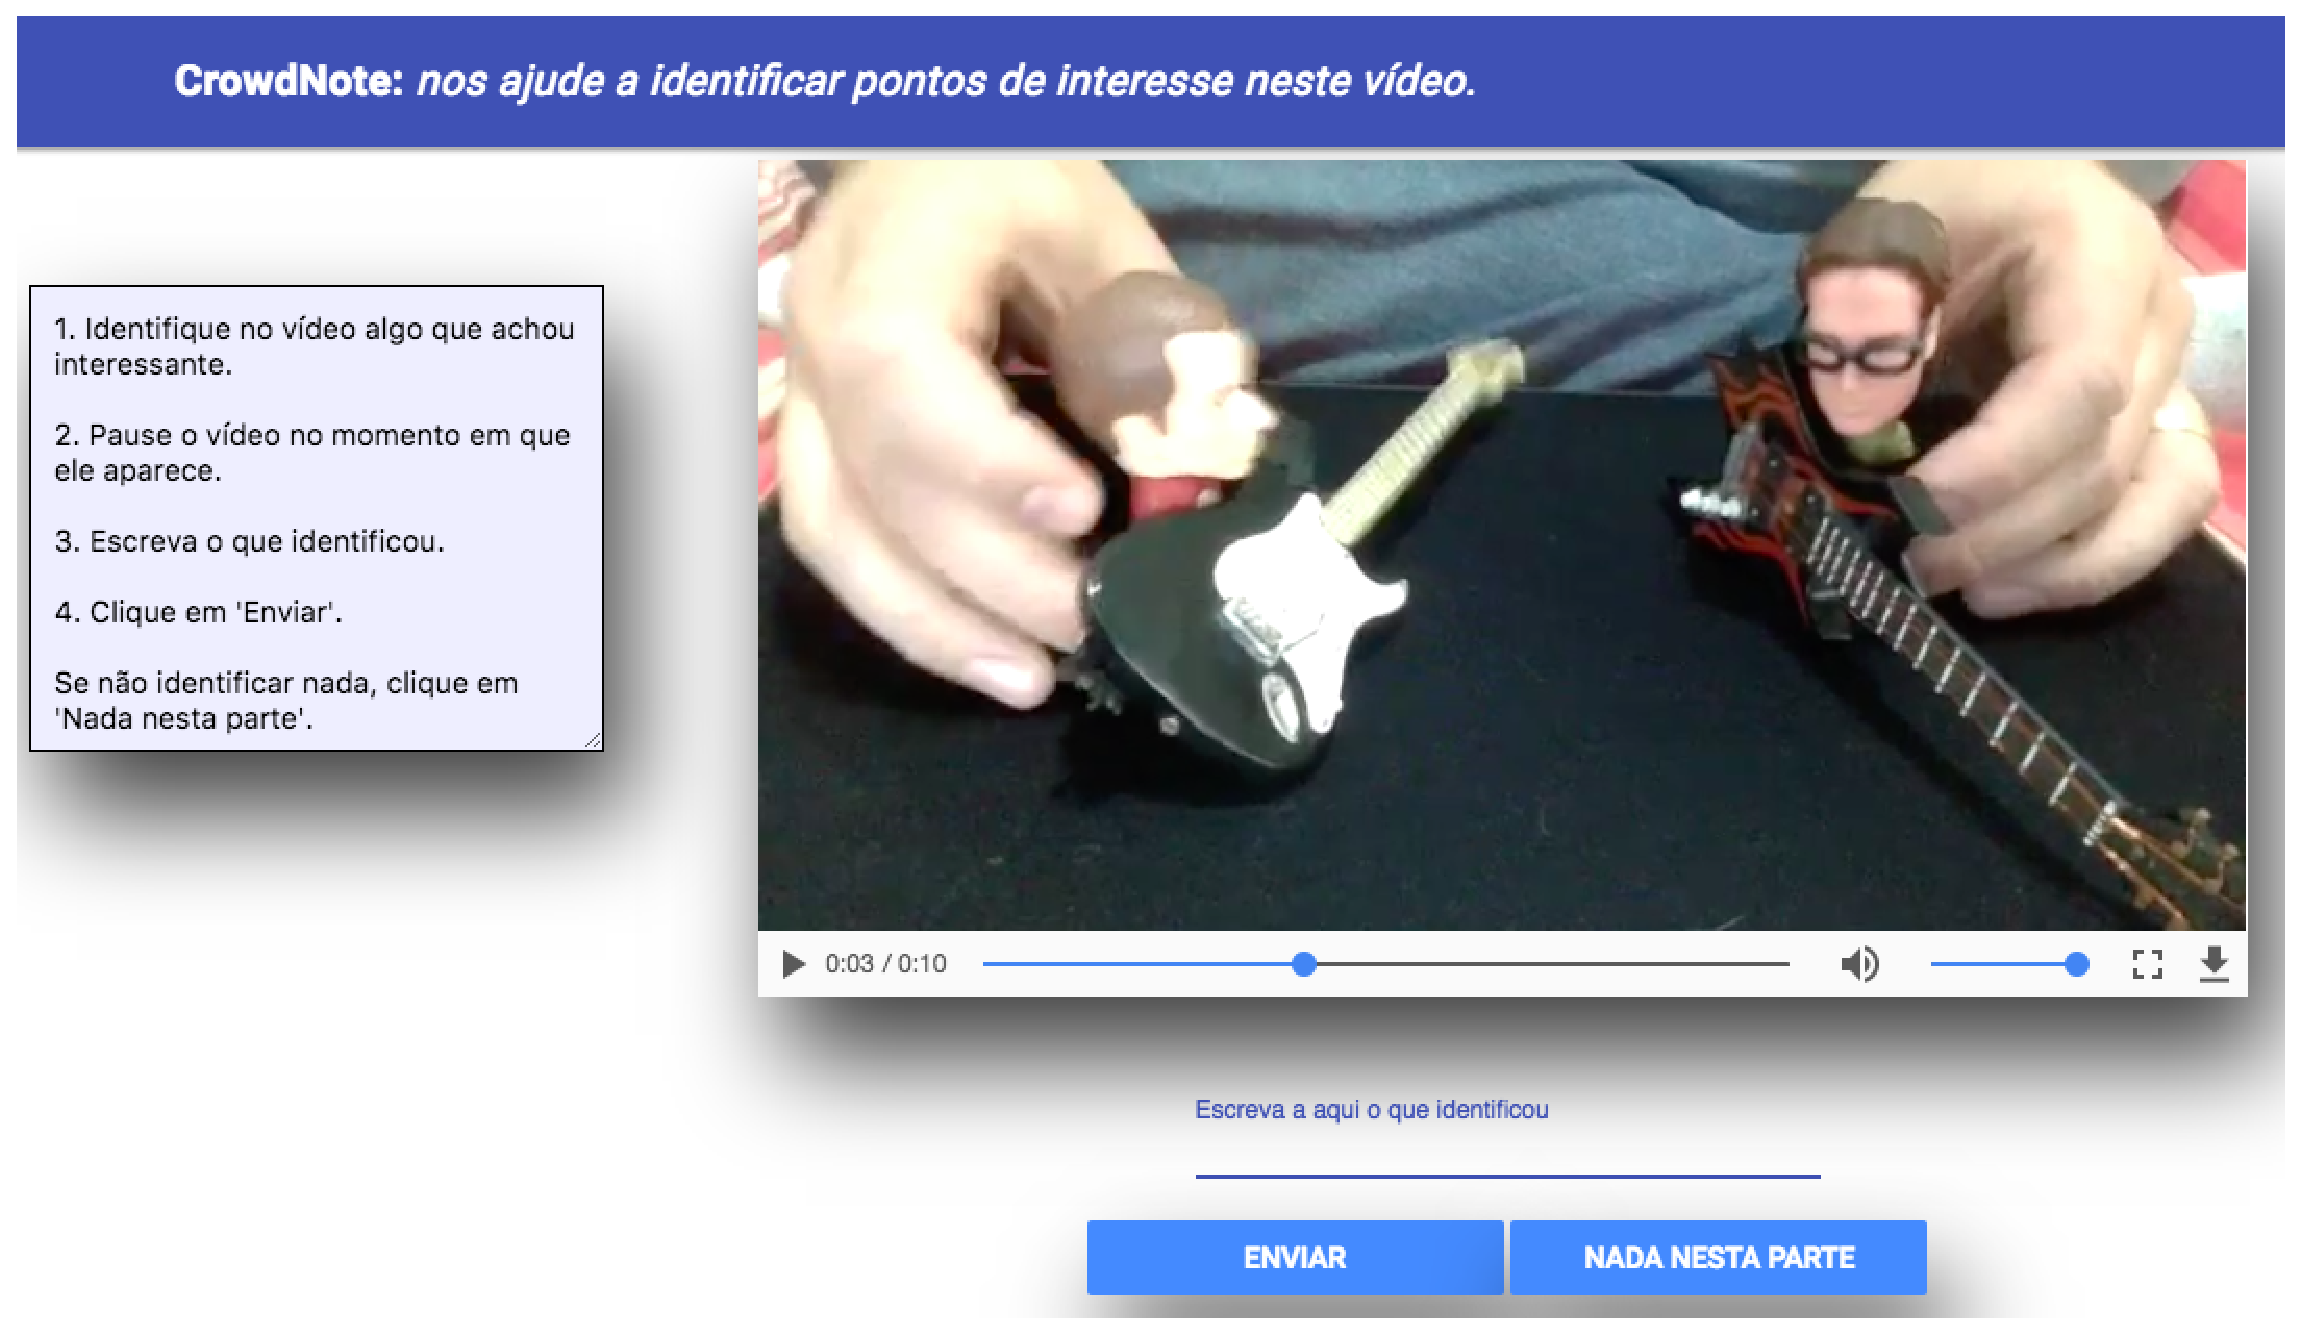
\includegraphics[scale=0.22] {figure/task_1}}
	\caption{Player}
	\label{player}
\end{figure}

When the user clicks on some extra content displayed in the video, the presentation is paused and a larger preview for the selected content is displayed in the zoom box as shown in the Figure~\ref{zoom}. This systems features navigation by extra-content instead the traditional timeline navigation, making available a button-bar with buttons to navigate among the extra contents.
 
\begin{figure}[h!]
	\centerline{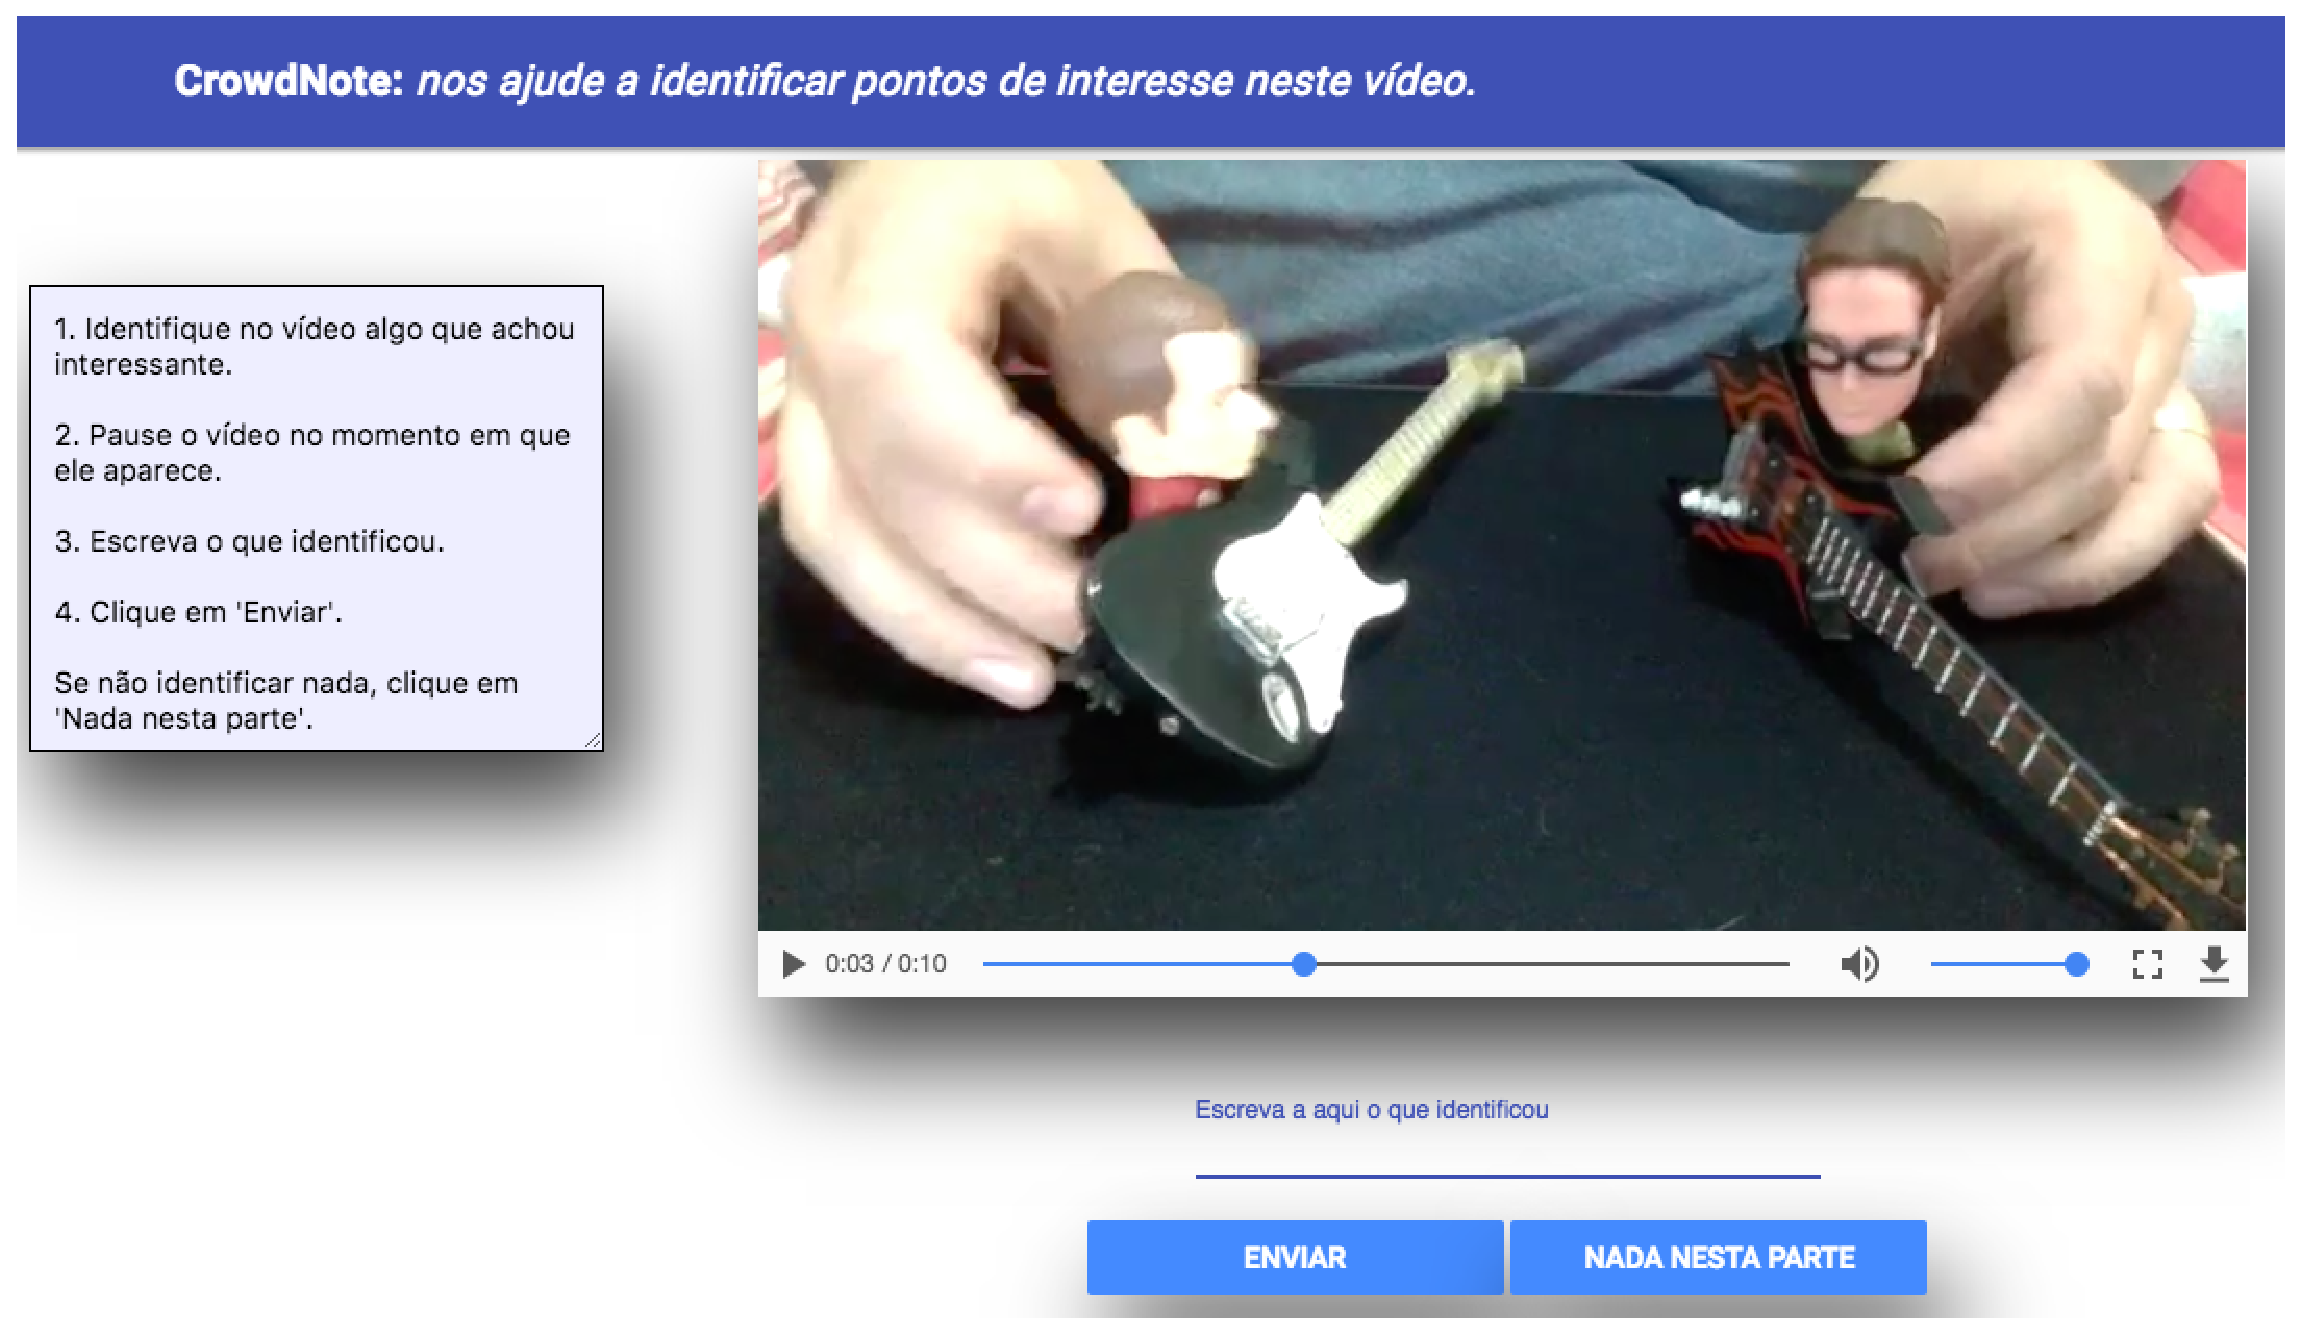
\includegraphics[scale=0.22] {figure/task_1}}
	\caption{Player}
	\label{zoom}
\end{figure}
